\documentclass{beamer}

\usepackage{amssymb,amsmath}
\usepackage{graphicx}
\usepackage{url}
\usepackage{color}
\usepackage{relsize}		% For \smaller
\usepackage{url}			% For \url
\usepackage{epstopdf}	% Included EPS files automatically converted to PDF to include with pdflatex

%For MindMaps
% \usepackage{tikz}%
% \usetikzlibrary{mindmap,trees,arrows}%

%%% Color Definitions %%%%%%%%%%%%%%%%%%%%%%%%%%%%%%%%%%%%%%%%%%%%%%%%%%%%%%%%%
%\definecolor{bordercol}{RGB}{40,40,40}
%\definecolor{headercol1}{RGB}{186,215,230}
%\definecolor{headercol2}{RGB}{80,80,80}
%\definecolor{headerfontcol}{RGB}{0,0,0}
%\definecolor{boxcolor}{RGB}{186,215,230}

%%% Save space in lists. Use this after the opening of the list %%%%%%%%%%%%%%%%
%\newcommand{\compresslist}{
%	\setlength{\itemsep}{1pt}
%	\setlength{\parskip}{0pt}
%	\setlength{\parsep}{0pt}
%}

%\setbeameroption{show notes on top}

% You should run 'pdflatex' TWICE, because of TOC issues.

% Rename this file.  A common temptation for first-time slide makers
% is to name it something like ``my_talk.tex'' or
% ``john_doe_talk.tex'' or even ``discrete_math_seminar_talk.tex''.
% You really won't like any of these titles the second time you give a
% talk.  Try naming your tex file something more descriptive, like
% ``riemann_hypothesis_short_proof_talk.tex''.  Even better (in case
% you recycle 99% of a talk, but still want to change a little, and
% retain copies of each), how about
% ``riemann_hypothesis_short_proof_MIT-Colloquium.2000-01-01.tex''?

\mode<presentation>
{
  % A tip: pick a theme you like first, and THEN modify the color theme, and then add math content.
  % Warsaw is the theme selected by default in Beamer's installation sample files.

  %%%%%%%%%%%%%%%%%%%%%%%%%%%% THEME
  %\usetheme{AnnArbor}
  %\usetheme{Antibes}
  %\usetheme{Bergen}
  %\usetheme{Berkeley}		% bem bacana - menu esquerdo
  %\usetheme{Berlin}
  %\usetheme{Boadilla}
  %\usetheme{boxes}
  %\usetheme{CambridgeUS}		% bem bacana - menu superior
  %\usetheme{Copenhagen}
  %\usetheme{Darmstadt}
  %\usetheme{default}
  %\usetheme{Dresden}
  \usetheme{Frankfurt}
  %\usetheme{Goettingen}
  %\usetheme{Hannover}		% bem bacana - menu esquerdo
  %\usetheme{Ilmenau}
  %\usetheme{JuanLesPins}
  %\usetheme{Luebeck}
  %\usetheme{Madrid}		%bacana
  %\usetheme{Malmoe}
  %\usetheme{Marburg}		% bem bacana - menu direito
  %\usetheme{Montpellier}
  %\usetheme{PaloAlto}		% bem bacana - menu esquerdo
  %\usetheme{Pittsburgh}
  %\usetheme{Rochester}		%bacana
  %\usetheme{Singapore}
  %\usetheme{Szeged}
  %\usetheme{Warsaw}

  %%%%%%%%%%%%%%%%%%%%%%%%%%%% COLOR THEME
  %\usecolortheme{albatross}		% azul escuro, massa
  %\usecolortheme{beetle}		% cinza, menu azul
  %\usecolortheme{crane}		% branco e amarelo, massa
  \usecolortheme{default}		% branco, azul clarinho
  %\usecolortheme{dolphin}		% azul e branco, legal
  %\usecolortheme{dove}			% cinza e branco, feio
  %\usecolortheme{fly}			% todo cinza, horrível
  %\usecolortheme{lily}			% parece o default
  %\usecolortheme{orchid}		% azul e branco, ok
  %\usecolortheme{rose}			% branco e violeta-claro, bonito
  %\usecolortheme{seagull}		% cinza, feio
  %\usecolortheme{seahorse}		% nhé, meio feio
  %\usecolortheme{sidebartab}		% Azul, branco, destaque na tab, interessante
  %\usecolortheme{structure}		% bichado
  %\usecolortheme{whale}		% Azul e branco, bem bonito

  %%%%%%%%%%%%%%%%%%%%%%%%%%%% OUTER THEME
  \useoutertheme{default}
  %\useoutertheme{infolines}
  %\useoutertheme{miniframes}
  %\useoutertheme{shadow}
  %\useoutertheme{sidebar}
  %\useoutertheme{smoothbars}
  %\useoutertheme{smoothtree}
  %\useoutertheme{split}
  %\useoutertheme{tree}

  %%%%%%%%%%%%%%%%%%%%%%%%%%%% INNER THEME
  \useinnertheme{circles}
  %\useinnertheme{default}
  %\useinnertheme{inmargin}
  %\useinnertheme{rectangles}
  %\useinnertheme{rounded}

  %%%%%%%%%%%%%%%%%%%%%%%%%%%%%%%%%%%

  \setbeamercovered{invisible} % or whatever (possibly just delete it)
  % To change behavior of \uncover from graying out to totally
  % invisible, can change \setbeamercovered to invisible instead of
  % transparent. apparently there are also 'dynamic' modes that make
  % the amount of graying depend on how long it'll take until the
  % thing is uncovered.

}


% Get rid of nav bar
\beamertemplatenavigationsymbolsempty

% Use short top
%\usepackage[headheight=12pt,footheight=12pt]{beamerthemeboxes}
%\addheadboxtemplate{\color{black}}{
%\hskip0.5cm
%\color{white}
%\insertshortauthor \ \ \ \ 
%\insertframenumber \ \ \ \ \ \ \ 
%\insertsection \ \ \ \ \ \ \ \ \ \ \ \ \ \ \ \ \  \insertsubsection
%\hskip0.5cm}
%\addheadboxtemplate{\color{black}}{
%\color{white}
%\ \ \ \ 
%\insertsection
%}
%\addheadboxtemplate{\color{black}}{
%\color{white}
%\ \ \ \ 
%\insertsubsection
%}

% Insert frame number at bottom of the page.
% \usefoottemplate{\hfil\tiny{\color{black!90}\insertframenumber}} 

\usepackage[english]{babel}
\usepackage[latin1]{inputenc}
\usepackage{subfigure}

\usepackage{times}
\usepackage[T1]{fontenc}

\usepackage{tikz}
\usetikzlibrary{arrows,shapes}
\tikzstyle{vertex}=[circle,fill=black!25,minimum size=10pt,inner sep=0pt]
\tikzstyle{blue vertex}=[circle,fill=blue!100,minimum size=10pt,inner sep=0pt]
\tikzstyle{red vertex}=[circle,fill=red!100,minimum size=10pt,inner sep=0pt]
\tikzstyle{edge} = [draw,thick,-]
\tikzstyle{red edge} = [draw, line width=5pt,-,red!50]
\tikzstyle{black edge} = [draw, line width=5pt,-,black!20]
\tikzstyle{weight} = [font=\smaller]

\title[GB21802]{GB21802 - Programming Challenges}
%\subtitle[]{Week 8 - String Problems}
\subtitle[]{Week 6 - String Problems}
\author[Claus Aranha]{Claus Aranha\\{\footnotesize caranha@cs.tsukuba.ac.jp}}
\institute{College of Information Science}
\date{2019-05-31,06-03\\{\tiny Last updated \today}}
\begin{document}

\section{Introduction}
\subsection{Title}
\begin{frame}
\maketitle
\vfill

\hfill{\tiny Suffix Trie pictures from ``Competitive Programming 3'' by Steven Halim}
\end{frame}

% \subsection{Notes from last week}
% \begin{frame}
  \frametitle{Results for the Previous Week}

  \begin{center}
    Here are the results for last week:

    \bigskip
    
    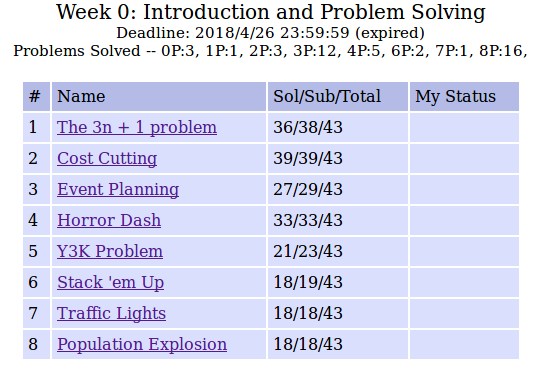
\includegraphics[width=0.8\textwidth]{img/resultW0}
    
    \bigskip

    Hope you enjoyed the warm up!
  \end{center}

\end{frame}

\begin{frame}[fragile]
  \frametitle{Comments from e-mails and questions -- 1}

  \begin{block}{Submission with Java}
    Two students had \structure{``runtime error''} with Java last week
    -- don't forget that your start class MUST be called {\bf Main}.
  \end{block}

  \vfill

\begin{verbatim}
class Main {
  public static void main(String[] args) {

    // do something...

  }
}
\end{verbatim}
\end{frame}

\begin{frame}
  \frametitle{Comments from e-mails and questions -- 2}
  \begin{block}{Input/Output}
    Two other students had problems because their program printed ``Please enter a number''.

    \bigskip

    You are very kind, but please {\bf follow the specifications} strictly!
  \end{block}
  
  \vfill

  \begin{block}{Format for MANABA submission}
    One student asked if the code for MANABA had to be the same as the code for UVA.

    \bigskip

    Yes. The code you submit on MANABA must be {\bf exactly the same}
    as the code you submitted for UVA.
  \end{block}
\end{frame}

\begin{frame}
  \frametitle{Short comments about the problems:}
  \begin{itemize}
  \item Cost Cutting, Event Planning, Horror Dash -- Easiest problems (find mean, find min, find min);
    \bigskip

  \item 3n+1 -- Still easy, but a few traps -- example of {\bf Memoization};
    \bigskip

  \item Y3K Problem -- Still easy, but skip year can be a bit troublesome.
    
  \end{itemize}
\end{frame}

%\begin{frame}
%  \frametitle{Comments about the problems}
%\end{frame}


\subsection{Outline}

\begin{frame}
  \frametitle{String Problems}
    \begin{exampleblock}{}
      String manipulation is very common in real life applications:

      \begin{itemize}
      \item Pre-processing of data for analysis; -- (JSON, CSV, Code)
      \item Bioinformatics; -- (Manipulation of symbols)
      \item Human Interfaces; -- (Text input/Output)
      \end{itemize}
    \end{exampleblock}

    \begin{block}{Characteristics of String Problems}
      \begin{itemize}
      \item Many ``parsing'' problems: special input, special output;
      \item Algorithms are usually derivated from DP;
      \item Special data structures for substrings;
      \end{itemize}
    \end{block}

    % This week, we will see some of these algorithms.
\end{frame}

\begin{frame}
  \frametitle{Ad-hoc (one-of-a-kind) string problems}
  Many String Problems in programming contests are {\bf "Ad-hoc"} (one-of-a-kind).
  They are usually a cover for problems of other types.

  \begin{exampleblock}{}
    \begin{itemize}
    \item \structure{Pre-processing/Parse}: Input data is in string, but
      the main problem is just numbers.\bigskip

    \item \structure{String Matching}: Compare two (or more) strings for
      similarities/differences. Find substrings.\bigskip

    \item \structure{Encode/Decode}: Transform encoded (encrypted)
      text into normal text (or vice-versa). Usually many solutions are
      possible (search for maximum solution).
    \end{itemize}
  \end{exampleblock}

  \bigskip

  Use of DP is very common!
\end{frame}

\section{String Basics}

\subsection{String Primer}

\begin{frame}[fragile]
  \frametitle{String Basic Operations: A primer (1)}
  {\smaller
    \begin{block}{String Representation}
      \begin{columns}[T]
        \column{0.45\textwidth}
\begin{verbatim}
// C/C++
char[100] str;
// ends with '\0'

#include<string>
str s;
\end{verbatim}
        \column{0.45\textwidth}
\begin{verbatim}
// JAVA
String str;

// JAVA strings
// are imutable!
\end{verbatim}
      \end{columns}
    \end{block}

    \begin{block}{Data Input}
      \begin{columns}[T]
        \column{0.45\textwidth}
\begin{verbatim}
// Word
scanf("%s",&str); cin >> str;

// Line
gets(str);
fgets(str,1000,strdin);
getline(cin,str);
\end{verbatim}
        \column{0.45\textwidth}
\begin{verbatim}
// Word
Scanner sc = new
       Scanner(System.in);
str = sc.next();

// Line
str = sc.nextLine();
\end{verbatim}
      \end{columns}
    \end{block}
  }
\end{frame}

\begin{frame}[fragile]
  \frametitle{String Basic Operations: A primer (2)}
  {\smaller
    \begin{block}{String Output and formatting}
      \begin{columns}[T]
        \column{0.45\textwidth}
\begin{verbatim}
// C/C++
printf("s = %s, l = %d\n",
   str, (int) strlen(str));
cout << "s = " << str <<
   ", l= " << str.length()
   << endl;
\end{verbatim}
        \column{0.45\textwidth}
\begin{verbatim}
// JAVA
System.out.print("..."); OR
System.out.println(); OR
System.out.printf(
   "s = %s, l= %d\n", str,
   str.length();)
\end{verbatim}
      \end{columns}
    \end{block}
    \begin{block}{Testing Two Strings for Equality}
      \begin{columns}[T]
        \column{0.45\textwidth}
\begin{verbatim}
result = strcmp(str,"test");
result = (str == "test");
\end{verbatim}
        \column{0.45\textwidth}
\begin{verbatim}
result =
   str.equals("test");

\end{verbatim}
      \end{columns}
    \end{block}
  }
\end{frame}

\begin{frame}[fragile]
  \frametitle{String Basic Operations: A primer (3)}
  {\smaller
    \begin{block}{Combining Two or More Strings}
      \begin{columns}[T]
        \column{0.45\textwidth}
\begin{verbatim}
// C/C++
strcpy(str,"hello");
strcat(str," world");
str = "hello";
str.append(" world");
\end{verbatim}
        \column{0.45\textwidth}
\begin{verbatim}
// JAVA
str = "hello";
str += " world";
// Careful!
// Creates new strings
\end{verbatim}
      \end{columns}
    \end{block}
    \begin{block}{Editing/Testing single characters in a string}
      \begin{columns}[T]
        \column{0.45\textwidth}
\begin{verbatim}
#include <ctype.h>
for (int i=0;str[i];i++)
   str[i] = toupper(str[i])
\end{verbatim}
        \column{0.45\textwidth}
\begin{verbatim}
// Java Strs are immutable
// create a new string
// or use StringBuffer
\end{verbatim}
      \end{columns}
    \end{block}
  }
\end{frame}

\begin{frame}[fragile]
  \frametitle{String Basic Operations: A primer (4)}
  {\smaller
    \begin{block}{String Tokenizer -- Separates a string based on a character}
      \begin{columns}[T]
        \column{0.45\textwidth}
\begin{verbatim}
// C/C++
#include <string.h>
for (char *p.strtok(str," ");
     p; p=strtok(NULL," "))
   printf("%s",p)

#include <sstream>
stringstream p(str);
while (!p.eof()) {
  string token;
  p >> token;
  }
\end{verbatim}
        \column{0.45\textwidth}
\begin{verbatim}
// JAVA
import java.util.*;
StringTokenizer st = new
  StringTokenizer(str," ");
while (st.hasMoreTokens())
  System.out.println(
     st.nextToken());
\end{verbatim}
      \end{columns}
    \end{block}
    }
\end{frame}

\begin{frame}[fragile]
  \frametitle{String Basic Operations: A primer (5)}
  {\smaller
    \begin{block}{Finding a Substring in a String}
      \begin{columns}[T]
        \column{0.45\textwidth}
\begin{verbatim}
// C/C++
char *p=strstr(str,substr);
if (p) printf("%d",p-str-1);

int pos=str.find(substr);
if (pos!=string::npos)
  cout << pos-1 << endl;
\end{verbatim}
        \column{0.45\textwidth}
\begin{verbatim}
// JAVA
int pos =
  str.indexOf(substr);
if (pos != -1)
  System.out.println(pos);
\end{verbatim}
      \end{columns}
    \end{block}
    \begin{block}{Sorting Characters in a string}
      \begin{columns}[T]
        \column{0.45\textwidth}
\begin{verbatim}
#include <algorithm>
sort(s, s+(int)strlen(s));
sort(s.begin(),s.end());
\end{verbatim}
        \column{0.45\textwidth}
\begin{verbatim}
//Immutable, break the
//string using
//toCharArray()
\end{verbatim}
      \end{columns}
    \end{block}
  }
\end{frame}

\begin{frame}[fragile]
  \frametitle{String Basic Operations: A primer (6)}
  {\smaller
    \begin{block}{Sorting an array of strings or characters}
      \begin{columns}[T]
        \column{0.45\textwidth}
\begin{verbatim}
// C/C++
#include <algorithm>
#include <string>
#include <vector>
vector<string> s;
// strings are put into s
sort(s.begin(), s.end())
\end{verbatim}
        \column{0.45\textwidth}
\begin{verbatim}
// JAVA
Vector<String> s =
   new Vector<String>();
Collections.sort(S);

\end{verbatim}
      \end{columns}
    \end{block}
  }
\end{frame}

\subsection{Ad-Hoc Problem Discussion}

\begin{frame}
  \frametitle{Discussion of Ad-hoc problems}

    \begin{exampleblock}{Problem 1 -- Immediate decodability}
      Given a set of {\bf 2 to 8 binary words}, of length
      between {\bf 1 and 10}, decide if the set is {\bf immediately
      decodable}. \bigskip

      A set is immediately decodable if {\bf no word is a prefix of
      another word}.
    \end{exampleblock}

    \begin{columns}
      \column{0.5\textwidth}
      {\bf Input example 1}
      \begin{itemize}
        \item 001
        \item 110
        \item 10101
        \item 01101
        \item 100
      \end{itemize}
      \column{0.5\textwidth}
      {\bf Input example 2}
      \begin{itemize}
        \item 001
        \item 110
        \item 10101
        \item 01101
        \item 10
      \end{itemize}
    \end{columns}\bigskip

    What is the brute force algorithm? What is the complexity? What
    is a smarter algorithm?
\end{frame}


\begin{frame}
  \frametitle{Discussion of Ad-hoc problems}
    \begin{exampleblock}{Problem 2 -- Caesar Cypher}
      {\small A {\bf rotational cypher} transforms \emph{plaintext} to
      \emph{cyphertext} by adding a constant value "k" to every character.\medskip

      Example: I LOVE YOU + ($k = 3$) $\rightarrow$ LCORYHCARY\medskip

      Given a dictionary of plaintext, find the best translation of
      the cyphertext.}
    \end{exampleblock}

    \begin{columns}
      \column{0.5\textwidth}
      {\small
      THIS\\
      DAWN\\
      THAT\\
      THE\\
      ZORRO\\
      OTHER\\
      AT\\
      THING\\
      \#\\
      BUUBDLA PSSPABUAEBXO}
      \column{0.5\textwidth}
      {\bf Output}:\\ ATTACK ZORRO AT DAWN
    \end{columns}
\end{frame}


\begin{frame}[fragile]
  \frametitle{Discussion of Ad-hoc problems}

    \begin{exampleblock}{Problem 3 -- Ensuring Truth}
      Given a boolean formula in the following format, is the formula
      {\bf satisfiable}?

      \begin{equation*}
        (x_1\land \hat{x_2}\land \ldots \land {x_n}) \lor (x_i\land \hat{x_j}\land\ldots) \lor \ldots
      \end{equation*}

      {\bf Examples:}
\begin{verbatim}
(a&b&c)|(a&b)|(a)        <--- Satisfiable;
(x&~x)                   <--- Not satisfiable;
\end{verbatim}
    \end{exampleblock}

    \begin{itemize}
      \item A big part of the program is to build a function to read a string with size over 5000 in the right format.
      \item SAT is a very hard problem, but for this particular string format, is there a simple way to calculate satisfiability?
    \end{itemize}
\end{frame}


\section{String Matching} % (6.4)
\subsection{Definition}

\begin{frame}
  \frametitle{String Matching}

  {\smaller
  \begin{block}{}
    Many String problems include some form of \structure{string matching}

    \medskip

    Find a substring $P$ inside of string $T$.
  \end{block}
  \begin{itemize}
  \item $P$ = OBEY
  \item $T$ = ASPBOBEBLEOLB\alert{OBEY}EYBEOLBEAY
  \end{itemize}

  \bigskip

  \begin{block}{}
    \begin{itemize}
    \item The easiest solution: Use strstr from the standard library!
    \item But... what if the search has special conditions?
    \begin{itemize}
      \item {\bf example:} O and 0 are the same character
    \end{itemize}
    \item Let's study how to make a string matching algorithm!
    \end{itemize}
  \end{block}

  {\bf First:} What is the complexity of a Complete search?

  }
\end{frame}

\begin{frame}[fragile]
  \frametitle{String Matching: Naive Algorithm}

  {\bf Complete search approach:} For every character $n[i]$, test if
  substring $m$ begins there.\bigskip

  \begin{exampleblock}{}
\begin{verbatim}
int naiveMatching() {
  for (int i = 0; i < n; i++)
    bool found = true;
    for (int j = 0; j < m && found; j++)
      if (i+j >= n || M[j] != N[i+j])
        found = false;
    if (found)
      printf("Found at index %d\n",i)
\end{verbatim}
  \end{exampleblock}
    \bigskip
    \begin{itemize}
      \item Average case: $O(n)$
      \item Worst case: $O(mn)$\\M = AAAAB, N = AAAAAAAAAAAAAAAAAB
      \item Why is this case bad?
    \end{itemize}
\end{frame}

\subsection{Knuth-Morris-Pratt}
\begin{frame}[fragile]
  \frametitle{The Knuth-Morris-Pratt (KMP) Algorithm}

  \begin{block}{Basic Idea}
    The KMP algorith will never re-match a character in $M$ that was
    matched in $N$.

    \bigskip

    If KMP finds a mismatch, it will skip $n$ to $m+1$, and rewind $m$ to the
    appropriate value to continue the match.
  \end{block}

\begin{verbatim}
N = COLIN COMBWELL CALLED A CO-CO-CO-COMBO BREAKER
M = CO-COMBO
    COXXXX
          COXXXXXXX
                   CXXXXXXXX
                            CO-COX
                               CO-COX
                                  CO-COMBO
\end{verbatim}
\end{frame}


\begin{frame}[fragile]
  \frametitle{The Knuth-Morris-Pratt (KMP) Algorithm}
    \begin{block}{How it works}

      The KMP needs to construct a ``M rewinded table'' $b$. When a mismatch happens, the substring $M$ is rewinded, but the $N$ index always moves forward.

\begin{verbatim}
M =  0 1 2 3 4 5 6 7      <-- Substring index
     C O - C O M B O
b = -1 0 0 0 1 2 0 0      <-- M "rewind" index
\end{verbatim}

If a miss happens at $m=5$ (M), the algorithm will return the M counter (j)
to $j = b[5] = 2$.
    \end{block}
\end{frame}

\begin{frame}[fragile]
  \frametitle{The Knuth-Morris-Pratt (KMP) Algorithm -- Code}
  {\smaller
  \begin{exampleblock}{}
\begin{verbatim}
char N[MAX_N], M[MAX_N];
int b[MAX_N], n, m;

void kmpPreprocess() {
  int i = 0, j = -1; b[0] = -1;
  while (i < m) {
     while (j >= 0 && M[i] != M[j]) j = b[j];
     i++; j++;
     b[i] = j; }}

void kmpSearch() {
  int i = 0, j = 0;
  while (i < n) {
     while (j >= 0 && N[i] != M[j]) j = b[j];
     i++; j++;
     if (j == m) {
        printf("M is found at index %d in N\n", i-j);
        j = b[j]; }}}
\end{verbatim}
  \end{exampleblock}
  }
\end{frame}

\section{String with DP} % (6.5)
\subsection{DP}
\begin{frame}
  \frametitle{String Processing with Dynamic Programming}
  \begin{block}{}
    Some string problems can be explained as a \structure{search}
    problem. In this case, we can solve them using Dynamic Programming.\bigskip

    \begin{itemize}
    \item String Alignment/Edit Distance
    \item Longest Common Subsequence
    \end{itemize}
  \end{block}
  \bigskip
\end{frame}

\subsection{Edit Distance}
\begin{frame}[fragile]
  \frametitle{String DP: Edit Distance}
  \begin{block}{}
    The {\bf Edit Distance}, {\bf String Alignment} or {\bf Levenhstein
    Distance}, consists of measuring how many spaces are needed to {\bf
    minimize the difference between two strings}.\bigskip

\begin{verbatim}
S1: ACAATCC -> A_CAATCC -> A_CAATCC
S2: AGCATGC -> AGCATGC_ -> AGCA_TGC
Diff:       -> +.++--+. -> +.++.+-+
\end{verbatim}\bigskip

  To maximise score, we want to avoid {\bf letter mismatches}.
  \end{block}

  {\bf Uses}
  \begin{itemize}
    \item Finding similar words.
    \item Identifying Mispellings.
  \end{itemize}
\end{frame}


\begin{frame}[fragile]
  \frametitle{String DP: Edit Distance}
  \begin{block}{Score Maximization Problem}
    Align two strings, $A$ and $B$, with the maximum alignment score.
    For each pair of characters, we have three choices:

    \begin{itemize}
    \item A[i] and B[i] are the same character ( '+': +2 score)
    \item A[i] and B[i] are diff character ('-': -1 score)
    \item Add a space to A[i] or B[i] ('.': -1 score)
    \end{itemize}
  \end{block}

\begin{verbatim}
S1: ACAATCC -> A_CAATCC         -> A_CAATCC
S2: AGCATGC -> AGCATGC_         -> AGCA_TGC
Diff:       -> 2-22--2- = +4    -> 2-22-2-2 = +7
\end{verbatim}

Trying all combinations: ($O(3^n)$). Let's try DP.
\end{frame}

\begin{frame}
  \frametitle{Edit Distance: Bottom Up DP Approach -- Setup}
  \begin{block}{State table}
    The state table $V$ has dimensions \emph{size(A)} by \emph{size(B)}
    \smallskip

    $V[i][j]$ is the maximum score for matching \emph{substrings} A[1..i], B[1..j].
  \end{block}
  \begin{exampleblock}{Initial Conditions}
    \begin{itemize}
    \item $V(0,0) = 0$ -- Empty Strings
    \item $V(i,0) = i*-1$ -- Fill "B" with "\_"
    \item $V(0,j) = j*-1$ -- Fill "A" with "\_"
    \end{itemize}
  \end{exampleblock}
\end{frame}

\begin{frame}
  \frametitle{Edit Distance: Bottom Up DP Approach -- Update}
  \begin{block}{State table}
    The state table $V$ has dimensions \emph{size(A)} by \emph{size(B)}
    \smallskip

    $V[i][j]$ is the maximum score for matching \emph{substrings} A[1..i], B[1..j].
  \end{block}
  \begin{exampleblock}{Transition Rule:}
    Score($C_1,C_2$) is the score of matching characters $C_1$ and $C_2$.\bigskip


    {\bf Update:}$V(i,j) = $ max(\emph{option1},\emph{option2},\emph{option3})
    \begin{itemize}
    \item option1 = V(i-1,j-1) + Score(A[i],B[j]) // Match or mismatch
    \item option2 = V(i-1,j) + Score(A[i],\_) // Delete A[i]
    \item option3 = V(i,j-1) + Score(\_,B[j]) // Insert B[j]
    \end{itemize}
  \end{exampleblock}
\end{frame}

\begin{frame}
  \frametitle{Edit Distance: Bottom Up DP Approach -- Example}
  Match ACAATCC and AGCATGC with a table.

\end{frame}
% TODO: Add table here.


\subsection{Longest Common Subsequence}

\begin{frame}[fragile]
  \frametitle{Problem 2 -- Longest Common Subsequence}
  {\smaller
    \begin{block}{Problem Definition}
      Given two strings $A$ and $B$, what is the longest common
      subsequence between them?

      \medskip

      Example:
\begin{verbatim}
String A:   'ACAATCC'     - A_CAAT_CC
String B:   'AGCATGC'     - AGCA_TGC_
Longest Common Subsequence: A_CA_T_C_

LCS: ACATC
\end{verbatim}
    \end{block}

    \begin{itemize}
    \item The LCS problem is similar to the String Alignment problem;
    \item The same DP algorithm presented before can be used;
    \item Set cost of Mismatch to $-\inf$, the cost of insert/deletion
      to 0, and the cost of matching to 1;
    \end{itemize}
  }
\end{frame}

\begin{frame}
  \frametitle{Longest Palindrome}
  {\smaller
    \begin{block}{Problem Description}
      Given a string $S$ of size up to $N = 1000$ characters, what is the
      longest palindrome that you can make by deleting characters from $S$?
    \end{block}

    Examples
    \begin{itemize}
    \item ADA\alert{M} -- ADA
    \item MADAM -- MADAM
    \item NEVERODDOREVEN\alert{ING} -- NEVERODDOREVEN
    \item RACE\alert{F1}CAR\alert{FAST} -- RACECAR
    \end{itemize}

  }
\end{frame}

\begin{frame}
  \frametitle{Longest Palindrome}
  {\smaller
    \begin{block}{Problem Description}
      Given a string $S$ of size up to $N = 1000$ characters, what is the
      longest palindrome that you can make by deleting characters from $S$?
    \end{block}

    DP Solution:
    \begin{itemize}
    \item State Table:
      {\smaller
      \begin{itemize}
      \item len(i,j) - The largest palindrome found between $i$ and $j$
      \end{itemize}}
    \item Start Conditions:
      {\smaller
      \begin{itemize}
        \item If $l=r$ then len$(l,r)=1$.
        \item If $r=l+1 \text{and} S[l]=S[r]$, len$(l,r)=2$, else len$(l,r)=1$.
      \end{itemize}}
    \item Transition:
      {\smaller
      \begin{itemize}
        \item If $S[l]=S[r]$, then len$(l,r)=2+\text{len}(l+1,r-1)$;
        \item else $\text{len}(l,r) = \text{max}(\text{len}(l+1,r),\text{len}(l,r-1))$
      \end{itemize}}
    \end{itemize}

    This DP has complexity $O(n^2)$

  }
\end{frame}

\begin{frame}[fragile]
  \frametitle{Longest Palindrome}

  Longest Palindrome DP: Diagonal Table Top Down

  {\smaller
\begin{verbatim}

       len(l,r)               len(l,r)         transition:
      final state           initial state   - A[l] == A[r]?
                                              len(l+1,r-1)+2
  R A C E F 1 C A R     R A C E F 1 C A R   - A[1] != A[r]?
                                              max(left,down)
R 1 1 1 1 1 1 3 5 7   R 1 1
A   1 1 1 1 1 3 5 5   A   1 1
C     1 1 1 1 3 3 3   C     1 1
E       1 1 1 1 1 1   E       1 1
F         1 1 1 1 1   F         1 1
1           1 1 1 1   1           1 1
C             1 1 1   C             1 1
A               1 1   A               1 1
R                 1   R                 1

\end{verbatim}

  }
\end{frame}


\section{Suffix Trie/Array} % (6.6)
\subsection{Outline}
\begin{frame}
  \frametitle{Suffix Trie: Definition}

  {\smaller
    \begin{block}{Definition}
      Data structure used to find matching suffixes of multiple strings.
    \end{block}

    \vfill

    \begin{center}
    \structure{Suffix Trie for \{'CAR','CAT','RAT'\}}
    \end{center}

    \vfill

    \begin{columns}[T]
      \column{0.25\textwidth}
      All Suffixes
      \begin{enumerate}
      \item CAR
      \item AR
      \item R
      \item CAT
      \item T
      \item RAT
      \item AT
      \item T
      \end{enumerate}
      \column{0.25\textwidth}
      Sorted, Unique Suffixes
      \begin{enumerate}
      \item AR
      \item AT
      \item CAR
      \item CAT
      \item R
      \item RAT
      \item T
      \end{enumerate}
      \column{0.45\textwidth}
      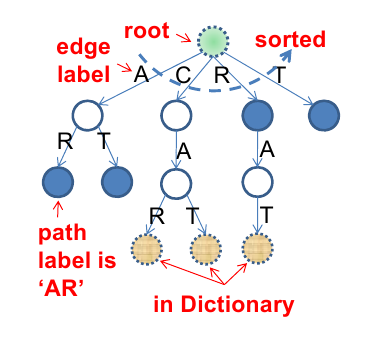
\includegraphics[width=.9\textwidth]{../img/suffixtrie_halim}\\
      % TODO: Replace suffix trie image with one of my own design
    \end{columns}
  }
\end{frame}

\begin{frame}
  \frametitle{Suffix Trie: Using it for a single, long string}
  {\smaller
  \begin{center}
    \structure{Suffix Trie (T='GATAGACA\alert{\$}')}
  \end{center}
  \begin{columns}[T]
    \column{0.35\textwidth}

    Create all $n$ suffixes:

    \begin{tabular}{c|l}
      i & suffix\\
      \hline
      0 & GATAGACA\$\\
      1 & ATAGACA\$\\
      2 & TAGACA\$\\
      3 & AGACA\$\\
      4 & GACA\$\\
      5 & ACA\$\\
      6 & CA\$\\
      7 & A\$\\
      8 & \$\\
    \end{tabular}

    Count the occurence of substring $m$:
    \begin{itemize}
    \item 'A': 4 times
    \item 'GA': 2 times
    \item 'AA': 0 times
    \end{itemize}
    \column{0.65\textwidth}
    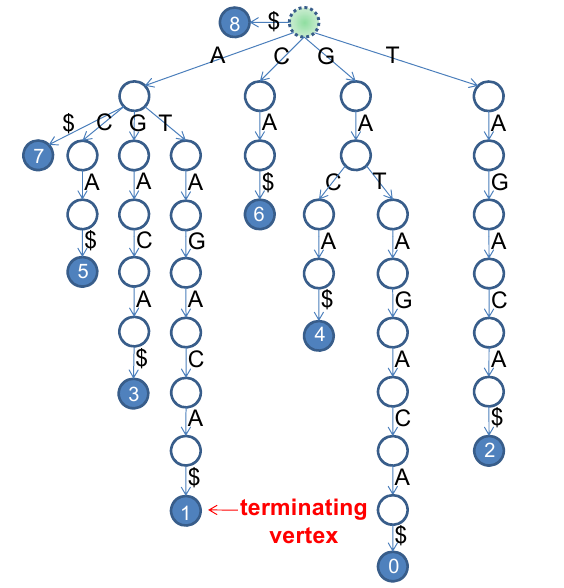
\includegraphics[width=.9\textwidth]{../img/suffixtrie_halim2}
  \end{columns}
  }
\end{frame}

\begin{frame}
  \frametitle{Suffix Trie: Suffix Tree}
  {\smaller
  \begin{center}
    \structure{Suffix Trie (T='GATAGACA\alert{\$}')}\\
    Compress single child nodes to obtain ``Suffix Tree''
  \end{center}
  \begin{columns}[T]
    \column{0.35\textwidth}

    \begin{tabular}{c|l}
      i & suffix\\
      \hline
      0 & GATAGACA\$\\
      1 & ATAGACA\$\\
      2 & TAGACA\$\\
      3 & AGACA\$\\
      4 & GACA\$\\
      5 & ACA\$\\
      6 & CA\$\\
      7 & A\$\\
      8 & \$\\
    \end{tabular}

    \bigskip

    With the suffix tree, many algorithms become faster.


    \column{0.65\textwidth}
    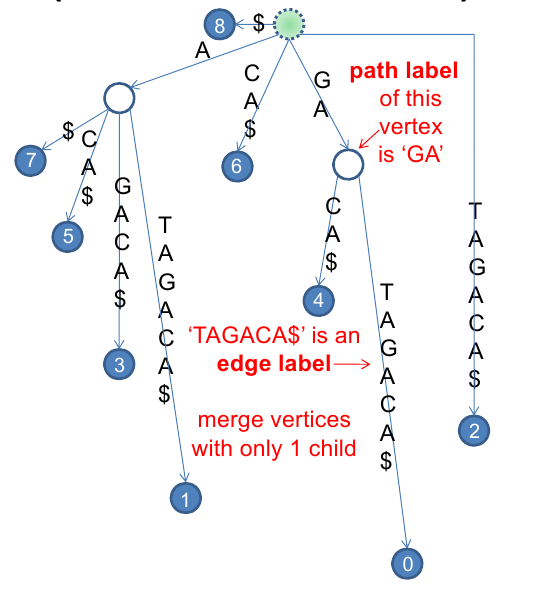
\includegraphics[width=.9\textwidth]{../img/suffixtree_halim}
  \end{columns}
  }
\end{frame}

\subsection{Uses of a Suffix Tree}
\begin{frame}
  \frametitle{Uses of a Suffix Tree 1: String Matching} {\smaller

    \structure{Assuming that we have the Suffix Tree already built},
    we can find all occurrences of substring $m$ in $T$ in time
    $O(m+\text{occ})$, where occ is the number of occurrences.

  \begin{center}
    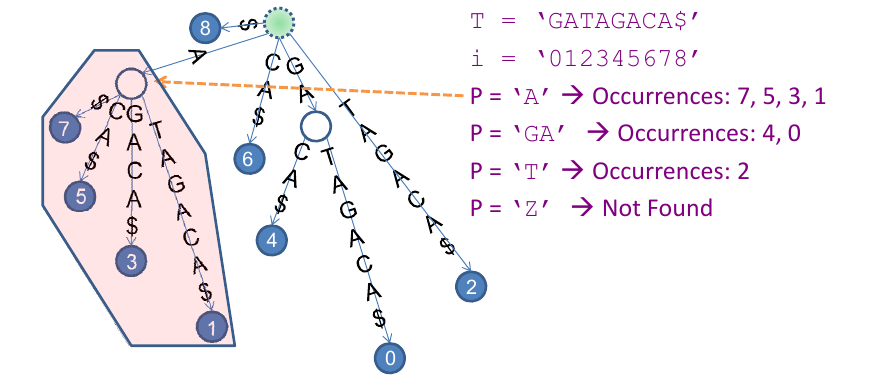
\includegraphics[width=0.9\textwidth]{../img/stringmatching_halim}
  \end{center}
  }
\end{frame}

\begin{frame}
  \frametitle{Uses of a Suffix Tree 2: Longest Repeated Substring}
  {\smaller
  \begin{itemize}
  \item The LRS is the longest substring with number of occurrences $> 2$;
  \item The LRS is the deepest internal node in the tree;
  \end{itemize}

  \begin{center}
    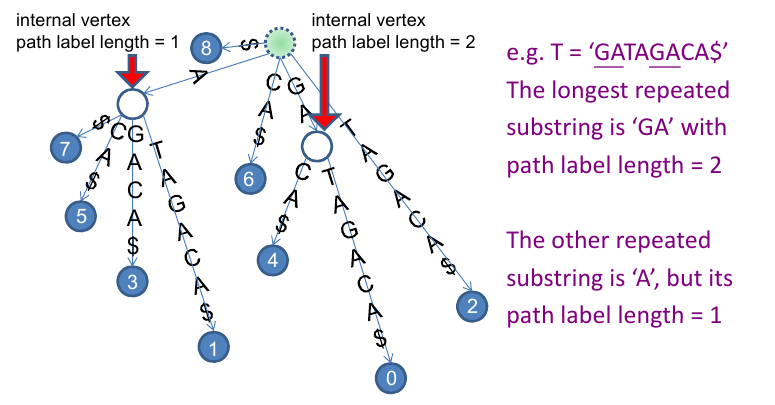
\includegraphics[width=0.9\textwidth]{../img/longestrepeatingsubstring_halim}
  \end{center}
  }
\end{frame}

\begin{frame}
  \frametitle{Uses of a Suffix Tree 3: Longest Common Substring}
  {\smaller
    \begin{itemize}
    \item We can find the common substring of $M$ and $N$ by making a
      combined Suffix Tree. Each string has a different ending
      character.
    \item The common substring is the deepest node that has both characters.
    \end{itemize}
  \begin{center}
    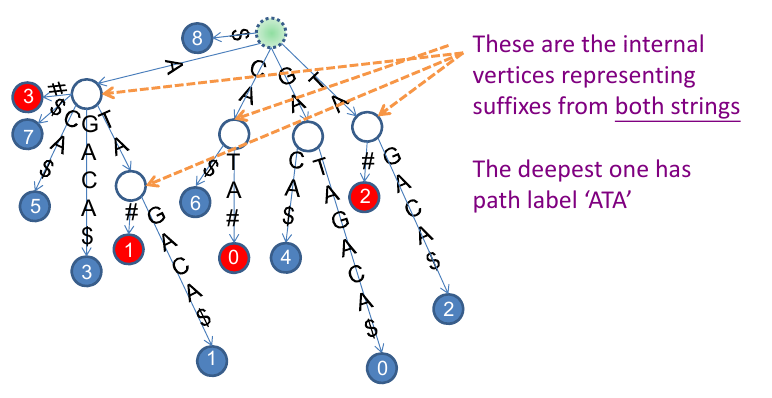
\includegraphics[width=0.9\textwidth]{../img/longestcommonsubstring_halim}
  \end{center}
  }
\end{frame}

\subsection{Suffix Array}
\begin{frame}
  \frametitle{Suffix Trie: Suffix Array (1)}
  {\small
  \begin{itemize}
    \item The algorithms in previous slides are very efficient...\\
      ... \structure{if you have the suffix tree}

      \medskip

    \item The suffix tree can be built in $O(n)$...\\
      ... but implementation is rather complex;

      \medskip

    \item In this course, we will see the \structure{Suffix Array};

      \medskip

    \item The Suffix Array is built in $O(n\log{n})$...\\
      ... but the implementation is very simple!
  \end{itemize}

  \vfill

  \begin{block}{}
    I encourage you to study the implementation of the suffix tree by yourself!
  \end{block}
  }
\end{frame}

\begin{frame}
  \frametitle{Suffix Trie: Suffix Array (2)}

  {\smaller

    \begin{itemize}
    \item To make a Suffix array, make an array of all possible
      suffixes of $T$, and sort it;
    \item The order of the suffix array is the
      \structure{visit in preorder} of the suffix tree;
      % TODO: Japanese for pre-order visit
    \item We can adapt all algorithms accordingly;
    \end{itemize}

  \begin{columns}
    \column{0.4\textwidth}
    \begin{tabular}{c|l}
      i & suffix\\
      \hline
      0 & GATAGACA\$\\
      1 & ATAGACA\$\\
      2 & TAGACA\$\\
      3 & AGACA\$\\
      4 & GACA\$\\
      5 & ACA\$\\
      6 & CA\$\\
      7 & A\$\\
      8 & \$\\
    \end{tabular}
    \column{0.2\textwidth}
    Sort $\rightarrow$
    \column{0.4\textwidth}
    \begin{tabular}{c|c|l}
      i & SA[i] & suffix \\
      \hline
      0 & 8 & \$\\
      1 & 7 & A\$\\
      2 & 5 & ACA\$\\
      3 & 3 & AGACA\$\\
      4 & 1 & ATAGACA\$\\
      5 & 6 & CA\$\\
      6 & 4 & GACA\$\\
      7 & 0 & GATAGACA\$\\
      8 & 2 & TAGACA\$\\
    \end{tabular}
  \end{columns}
  }
\end{frame}

\begin{frame}[fragile]
  \frametitle{Suffix Array: Implementation (1)}
  {\smaller
    \begin{exampleblock}{Simple Implementation}
\begin{verbatim}
#include <algorithm>
#include <cstdio>
#include <cstring>
using namespace std;
char T[MAX_N]; int SA[MAX_N],i,n;

bool cmp(int a, int b) { return strcmp(T+a, T+b) < 0; }
// O(n)

int main() {
  n = (int) strlen (gets(T));
  for (int i = 0; i < n; i++) SA[i] = i;
  sort (SA, SA+n, cmp); // O(n^2 log n) }
\end{verbatim}
    \end{exampleblock}

    This implementation is too slow for strings bigger than 1000 characters.
  }
\end{frame}

\begin{frame}[fragile]
  \frametitle{Suffix Array: Implementation (2.1)}
  {\smaller
    \begin{exampleblock}{O(n log n) implementation using ``ranking pairs/radix sort''}
\begin{verbatim}
char T[MAX_N]; int n; int c[MAX_N];
int RA[MAX_N], tempRA[MAX_N], SA[MAX_N], tempSA[MAX_N];

void countingSort(int k) {
  int i, sum, maxi = max(300,n); //255 ASCII chars or n
  memset(c, 0, sizeof(c));
  for (i = 0; i < n; i++) c[i+k<n? RA[i+k] : 0]++
  for (i = sum = 0; i < maxi; i++)
    { int t = c[i]; c[i] = sum; sum += t;} //frequency
  for (i = 0; i < n; i++)
    tempSA[c[SA[i]+k < n ? RA[SA[i]+k] : 0]++] = SA[i];
  for (i = 0; i < n; i++) // update suffix array
    SA[i] = tempSA[i];
}

// ... continues next slide
\end{verbatim}
    \end{exampleblock}
  }
\end{frame}

\begin{frame}[fragile]
  \frametitle{Suffix Array: Implementation (2.2)}
  {\smaller
    \begin{exampleblock}{O(n log n) implementation using ``ranking pairs/radix sort''}
\begin{verbatim}
// ... continued from last slide

void constructSA() {
  int i, k, r;
  for (i = 0; i < n; i++) { RA[i] = T[i]; SA[i] = i;}
  for (k = 1; k < n; k <<=1) {
    countingSort(k); countingSort(0);
    tempRA[SA[0]] = r = 0;
    for (i = 1; i < n; i++) tempRA[SA[i]] =
           (RA[SA[i]] == RA[SA[i-1]] &&
            RA[SA[i]+k] == RA[SA[i-1]+k]) ? r : ++r;
    for (i = 0; i < n; i++)
      RA[i] = tempRA[i];
    if (RA[SA[n-1]] == n-1) break;
}}
\end{verbatim}
    \end{exampleblock}
  }
\end{frame}

\begin{frame}
  \frametitle{Suffix Array: Using Suffix Array (1)}
  {\smaller
    \begin{block}{String Matching: Finding 'GA'}
      \begin{itemize}
      \item Do a binary search once to find the lower bound;
      \item Do a binary search once to fint the upper bound;
      \end{itemize}
    \end{block}
    \begin{center}
      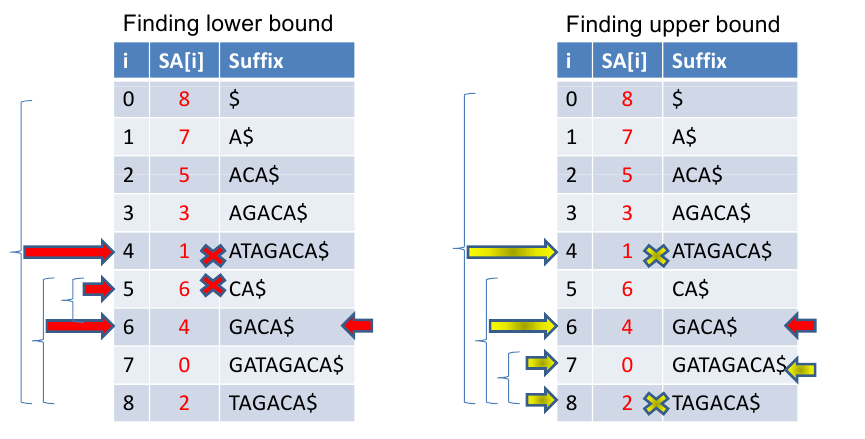
\includegraphics[width=0.9\textwidth]{../img/suffixarray_halim}
    \end{center}
  }
\end{frame}

\begin{frame}
    \frametitle{Suffix Array: Using Suffix Array (2)}
  {\smaller
    \begin{block}{Longest Repeated Substring}
      Find the longest common prefix between suffix $i$ and $i+1$
    \end{block}
    \begin{center}
      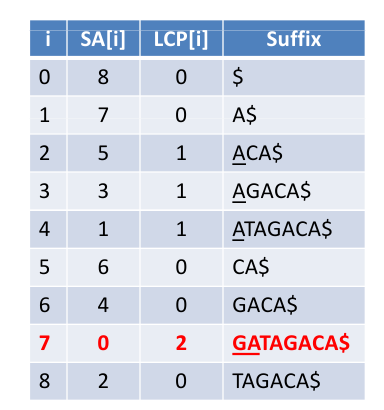
\includegraphics[width=0.5\textwidth]{../img/suffixarray2_halim}
    \end{center}
  }
\end{frame}

\begin{frame}
    \frametitle{Suffix Array: Using Suffix Array (3)}
  {\smaller
    \begin{block}{Longest Common Substring}
      \begin{itemize}
      \item Create Suffix Array for appended strings $MN$;
      \item Find the longest common prefix that has both string enders;
      \end{itemize}
    \end{block}
    \begin{center}
      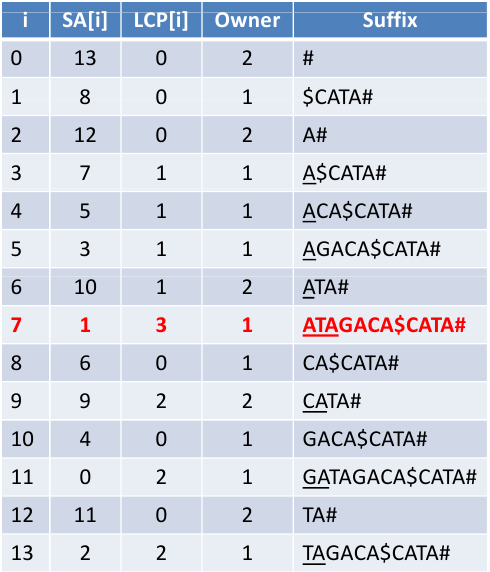
\includegraphics[width=0.45\textwidth]{../img/suffixarray3_halim}
    \end{center}
  }
\end{frame}

\section{Conclusion}

\subsection{Problem Discussion}
\begin{frame}
  \frametitle{This Week's Problems}
  \begin{itemize}
  \item Dominator
  \item Forwarding Emails
  \item Ordering
  \item Place the Guards
  \item Doves and Bombs
  \item Come and Go
  \item ACM Contest and Blackout
  \item Ancient Messages
  \end{itemize}
\end{frame}

\begin{frame}
  \frametitle{Problem Hints (0)}

  {\smaller
  \begin{block}{Library!}
    For many of these problems, you will use a lot of repeated code:
    \begin{itemize}
    \item Visited Node arrays;
    \item Adjacent lists;
    \item Parent nodes;
    \end{itemize}

    \bigskip

    Prepare a template for the most common codes you use, and
    copy-paste it whenever necessary!
  \end{block}
  \begin{block}{Tricky Cases}
    \begin{itemize}
    \item Graphs with 1 or 0 Vertex
    \item Unconnected Graphs
    \item Self Loops
    \item Double edges
    \end{itemize}
  \end{block}
  }
\end{frame}

\begin{frame}
  \frametitle{Problem Hints (1)}  
  {\smaller
    \begin{block}{Dominator}
      \begin{itemize}
        \item If All paths from 0 to node B pass through node A, then node A {\bf dominates} node B;
        \item For all pair of nodes $i,j$, output ``Y'' if $i$ {\bf dominates} $j$, or ``N'' if not;
      \end{itemize}
    \end{block}

    \bigskip

    The idea of this problem is one of ``reachability'' -- can I reach
    node $j$ if I remove node $i$ from the graph?

    \bigskip

    Note: if $j$ is not connected to ``0'', then \emph{no one dominates j}
  }
\end{frame}

\begin{frame}
  \frametitle{Problem Hints (2)}
  {\smaller
    \begin{block}{Forwarding Emails}
      Every person $i$ sends e-mail only to person $j$.
      
      \bigskip
      
      What is the longest email chain?
      
      \bigskip
      
      Where does it start?
    \end{block}
    
    \begin{itemize}
    \item How do you deal with loops?
    \item Time limit is not very large, Try to find an O(n) solution!
    \end{itemize} 
  }
\end{frame}

\begin{frame}
  \frametitle{Problem Hints (3)}
  {\smaller
    \begin{block}{Ordering}
      Print all possible Orderings of a Direct Acyclic Graph

      \bigskip

      Generalize the DAG ordering algorithm which we discussed in class.
    \end{block}
    
    \begin{block}{Palace Guards}
      \begin{itemize}
        \item How do you represent the roads and junctions as a Graph?
        \item Find a ``guard-no guard'' assignment to vertices of the
          graph.
        \item First test if a solution is possible!
      \end{itemize}
    \end{block}    
  }
\end{frame}

\begin{frame}
  \frametitle{Problem Hints (4)}
  {\smaller
    \begin{block}{Doves and Bombs}
      This problem is about finding ``critical vertices'' in a
      graph. But how do you calculate the ``pigeon value'' of a
      vertex?
    \end{block}

    \begin{block}{Come and Go}
      Straight implementation of ``Strong Connected Components''. Be
      careful with tricky graphs!
    \end{block}    
  }
\end{frame}

\begin{frame}
  \frametitle{Problem Hints (5)}
  {\smaller
    \begin{block}{ACM Contest and Blackout}
      Goal: Find the {\bf First} minimum spanning Tree and the {\bf
        Second} minimum spanning Tree
    \end{block}

    \bigskip
    
    \begin{itemize}
    \item In this class we discussed how to find the Minimum Spanning Tree      
    \item How would we find the {\bf second minimum?}
    \item Idea: Maybe if we remove some edges from the graph?
    \end{itemize}
  }
\end{frame}

\begin{frame}
  \frametitle{Problem Hints (6)}
  \begin{block}{Ancient Message -- Challenge problem!}
    Count the symbols inside an image -- order does not matter!

    \bigskip

    What is the {\bf Main} difference between the symbols?
  \end{block}
    
  \begin{itemize}
  \item The shape and size of the symbols is actually not important!
  \item Before you begin programming, discover what is the real
    difference between the symbols.
  \item Hint: The numbers ``1'', ``0'', ``8'' have the same difference.
  \end{itemize}    
\end{frame}


% \begin{frame}
%   \frametitle{Next Week}
%   \begin{itemize}
%   \item Final Class: Problems Remix
%   \item Class Evaluation
%   \item See you!
%   \end{itemize}
% \end{frame}

\end{document}
